\section*{Test 8 Allocation of demographic parameters}

The parameter analysis serves to represent the effects of the parameters used in the simulation. For the three-storey test floor plan illustrated in Figure 7, it should be demonstrated how the total evacuation time changes when the individual person parameters are varied. This is to be repeated for each individual parameter, with the other parameters set as fixed standard values. The parameter being tested should be the same for all persons once (e.g. speed of all persons 0.5 m/s, 0.75 m/s, 1.0 m/s,...) and varied once in a statistically equally distributed way around a fixed mean value (e.g. speed: 0.75 m/s, 0.5-1.0 m/s, 0.25-1.25 m/s,...).

\noindent
On the 2nd floor there are no more stairs upwards. It differs in this way from the 1st floor.


\begin{figure}[h]
	\centering
	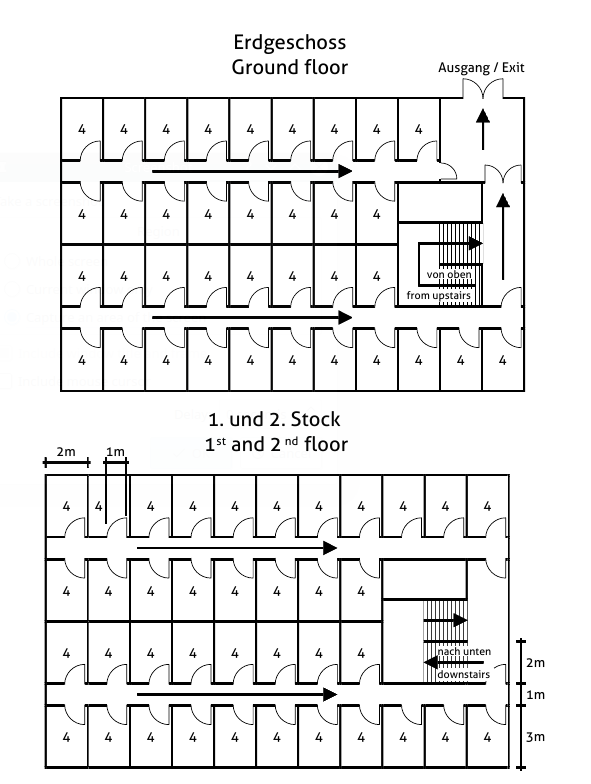
\includegraphics[scale=0.5]{test_description/Test_floor_plan_test_8.png}
	\caption{\footnotesize \textbf{Test floor plan for the systematic analysis of person parameters. Four persons should be located in each "room". Width of a wing of a door: 1 m}}
\end{figure}

